\documentclass[12pt]{article}
\usepackage{graphicx} % Required for inserting images
\usepackage{amsmath}
\usepackage[T1]{fontenc}
\usepackage{geometry}
\geometry{
 a4paper,
 total={170mm,257mm},
 left=20mm,
 top=20mm,
 }

 \begin{document}
	\bibliographystyle{IEEEtran}
	\vspace{3cm}

	\title{CS2323 - Lab 3 - RiscV Assembler Report}
	\author{Shiven Bajpai - AI24BTECH11030}

	\maketitle
	\bigskip    	

	\renewcommand{\thefigure}{\theenumi}
	\renewcommand{\thetable}{\theenumi}

	\tableofcontents
	\newpage

    \section{Preface}
    In this project I aimed to create an assembler that was fully RV64I Compatible. I wanted to implement pseudo instructions as well but due to time constraints I decided not to. I have learnt a lot over the course of this project and as a fresher I must say it was probably the most exciting thing I have worked on in college so far.
    \\

    In the end I had an assembler which had the following capabilities:
    \begin{itemize}
        \item Supports all RV64I Base Integer Instructions
        \item Is able to correctly handle whitespace and comments
        \item Is capable of handling literals in Decimal, Hex, Octal and Binary formats
        \item Gives clear error reporting including the Line number as well as type of issue.
        \item Has basic command line options for specifying custom file names and enabling debug information
    \end{itemize}

    \section{Approach to the Problem}

    The way I approached the problem was that I identified 3 simple steps that had to be performed for every instruction in the input:

    \begin{enumerate}
		\item{Read the instruction}
		\item{Convert it to binary}
		\item{Write the binary code to the output file/buffer}
	\end{enumerate}

    At first It seemed as though I could achieve this in a single loop iterating over all instructions. However there was the issue that if I were parsing the input sequentially it would not be possible for me to resolve a Label in one instruction that is declared on a later line. To remedy this problem I could've chosen to defer the processing of all instructions including labels to happen after processing all other instructions, however I chose a simpler approach where I performed two passes. One where I identified labels and the other where I actually processed the instructions.
    \\

    I also made some extra design decisions outside of the requirements of the problem statement, the justification for which is as follows:
    \\

    I chose to remove unnecessary whitespace in the first pass as well. Not only does this simplify the processing in the second pass, but also it provided me with an opportunity to create an intermediate cleaned up version of the code without labels and extra whitespace. My program write this intermediate version out to a separate file called "cleaned.s". The reason for this is that, inspired by the RIPES simulator, I wanted to have my simulator (in the next project) capable of showing a cleaned up version of the code separated by labels just like RIPES has in the middle pane of the Editor tab.

    \section{Code Implementation}

    The overall control flow of my program can be summarized as follows:
    \\\\

    \begin{figure}[h!]
        \centering
        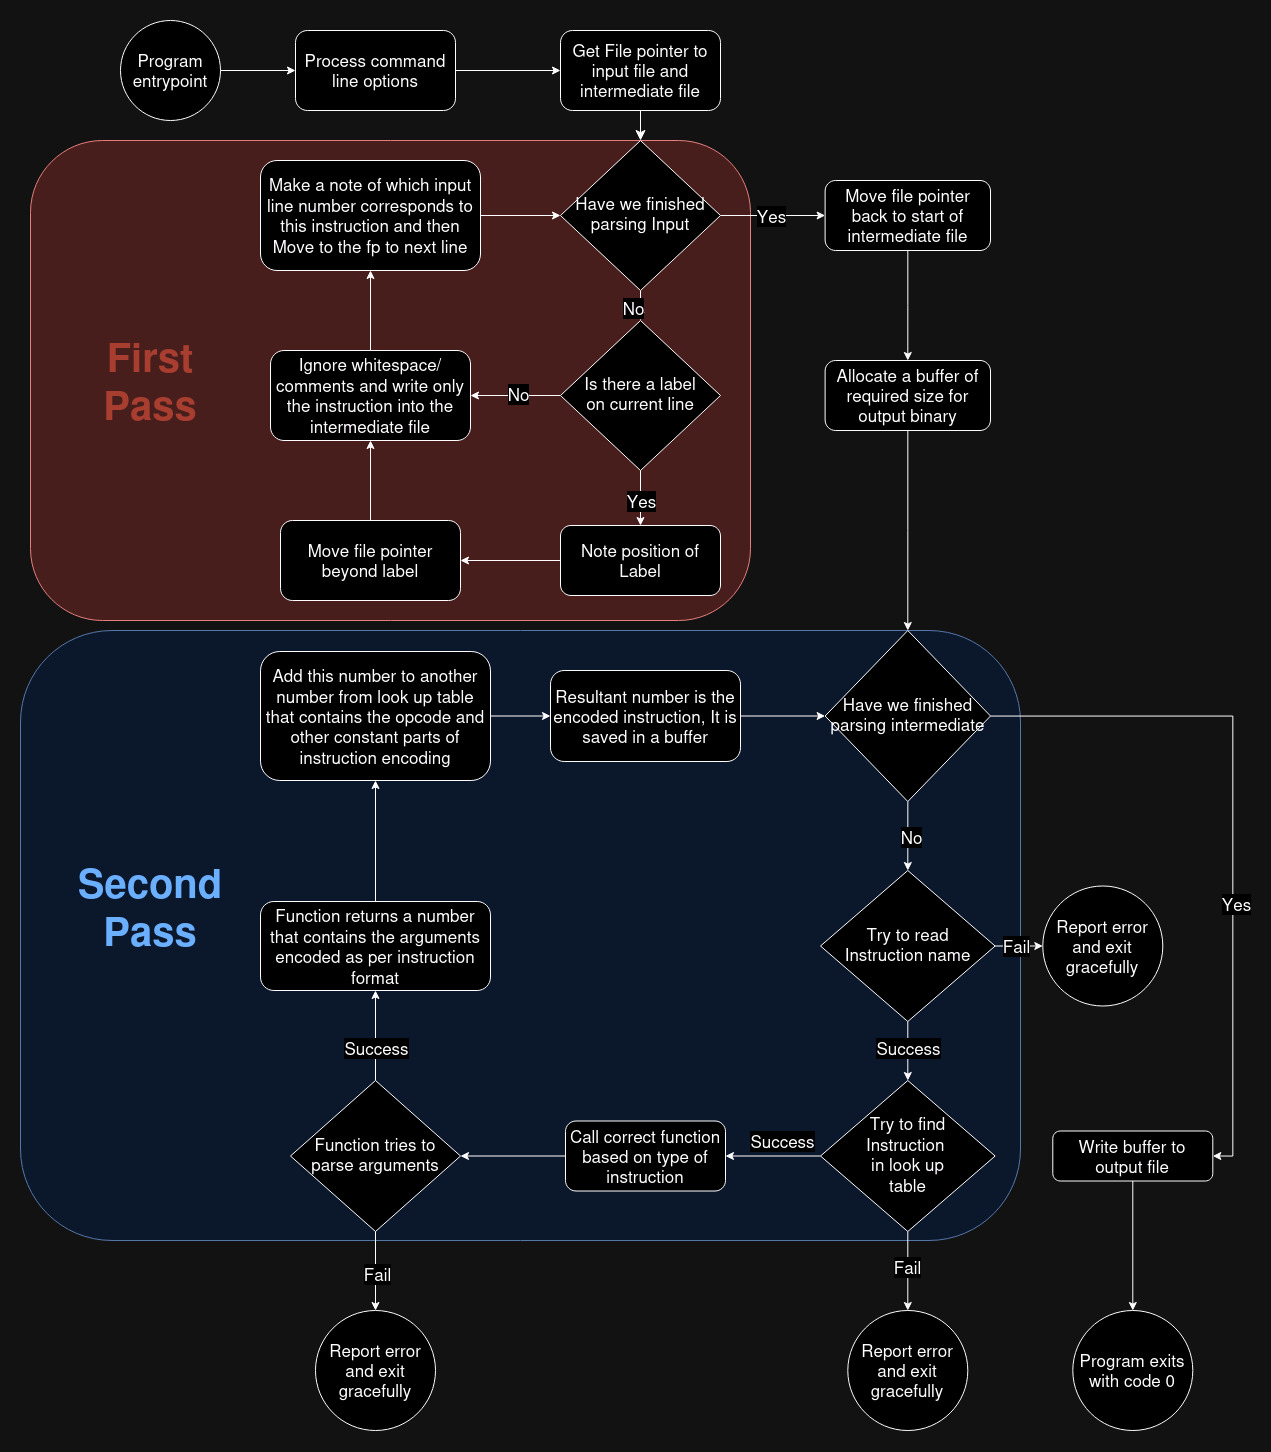
\includegraphics[width=1\linewidth]{Flowchart.png}
        \caption{Program Flowchart}
        \label{fig:flowchart}
    \end{figure}

    Note that to keep it clean, some checks for overflowing buffer size while reading instruction/Label names have been omitted from the flowchart. Essentially, if an instruction/label name is longer than 128 chars the program will declare it invalid and exit gracefully.
    \\

    \subsection{Noting Position of labels}
    In the first pass, to store information about labels as they are encountered, I use a struct called label\_index which is defined in \verb#index.c#. This struct is essentially a data structure that manages a pair of key and value arrays. Some helper functions are defined that take care of memory management and the function \verb#int label_to_position# performs a linear search over the data to convert labels to addresses
    
    \subsection{Instruction lookup tables}
    Information about the instructions is hard coded into the program in an array of structs containing the instruction name, a number corresponding constant bits set, and an enum value indicating which function is to be called to parse arguments. While parsing instructions this enum value is checked via a switch statement to call the right function. The lookup table is present in \verb#translator.c#
    \\

    I would like to note that for a large set of instructions it would be considerably faster to use a hashmap for such lookup operations, but since the size of instructions here was relatively small I chose to skip using a hashmap for simplicity.

    \subsection{Parsing Arguments}
    Arguments are parsed by individual functions that are uniquely defined for different types of instructions which have different formats of arguments, each of these unique functions simply calls a generalized function \verb#int* parse_args# with the right parameters based on the format, then performs some extra checks and transformations on the returned values to encode the arguments as per the instruction format and then returns this number.

    \subsection{Error Handling}
    Whenever an error is encountered, the program has three aims: Free memory, report the error and exit gracefully
    \\

    The error reporting is done immediately in whichever function the error is encountered. Then although it would be sufficient to simply exit the program there and let the OS de-allocate memory, In my program all functions return and indicate to the caller in some way or another that the function failed, which causes to caller to also free memory and return until the main function is reached which is where the program actually always exits.\\

    Since we are reading a cleaned up version of the input in the second pass, the line numbers may not match those in the input, so there is also a \verb|vec| struct called \verb|line_mapping| that is passed around that contains the mapping between instruction numbers and the line on which they appear in the input file

    \section{Testing}
    For testing, I used a small set of test cases comprising of:
    
	\begin{itemize}
		\item{The examples given with the problem statement}
		\item{My previous Lab assignments under this course}
		\item{A single program containing all instructions}
	\end{itemize}
	
 Testing is managed by a simple test harness written as a bash script in the tests directory\\
	To have a ``correct'' output to test against, I needed to use another known correct compiler. Since RIPES does not allow you to save the hex output I used an online riscv assembler at https://riscvasm.lucasteske.dev/ to generate a correct version to test against
	To run the tests one may use the `make run' command from the root directory.

    \iffalse
    \section{Learnings in Hindsight}
    Looking back after completing this project I have quite a few things I realized I could've done differently that I would like to quickly mention. 
    \begin{enumerate}
        \item I didn't need to free memory before exiting when an error was encountered because the OS does it anywys
        \item I could've used a more advanced approach using a lexer that would've given me more information allowing for better error reporting
        \item I did learn how to implement a hashmap for this project but then decided not to use it but maybe I could've done so.
    \end{enumerate}
    \fi

    \newpage
    \appendix
    \section*{Appendices}
    \addcontentsline{toc}{section}{Appendices}
    \renewcommand{\thesubsection}{\Alph{subsection}}
    
    \subsection{Usage Guide}

    \subsubsection*{How To build}
    \begin{enumerate}
        \item Run `make build` to compile the project, binary is produced in \verb#/bin# called \verb#riscv_asm#
        \item Run the binary. A temporary file called `cleaned.s` will be created and the machine code output shall be in `output.hex` in the same directory by default. 
    See the next section for how to specify input/output files
    \end{enumerate}
    
    \subsubsection*{Command line switches}
    \begin{verbatim}
`-d` 
`--debug`\end{verbatim}
    Runs the assembler in debug mode, providing more verbose output as it runs
    \\
    
    \begin{verbatim}
`-i <filename>`
`--input <filename>`\end{verbatim}
    Specifies a file for input, defaults to input.s if not specified
    \\
    
    \begin{verbatim}
`-o <filename>`
`--output <filename>`\end{verbatim}
    Specifies a file for output, defaults to output.hex if not specified

    \newpage
    \subsection{Project File Structure}

    \begin{verbatim}
.
+-- root
    +-- bin/                    (Contains output binary when built)
    +-- build/                  (Object files are placed here)
    +-- report/
    |   +-- AI24BTECH11030.tex  (The latex file for project report)
    +-- src/
    |   +-- index.c             (Defines label_index struct)
    |   +-- index.h
    |   +-- main.c              (Main file)
    |   +-- translator.c        (Contains most functions and hard-coded data 
    |   |                        regarding instruction parsing)
    |   +-- translator.h
    |   +-- vec.c               (Defines the vec struct)
    |   +--  vec.h
    +-- tests/
    |   +-- cases/              (The actual tests cases are stored here)
    |   |   +-- (...)
    |   +-- outputs/            (Program output from running tests goes here)
    |   +-- test.bash           (Basic Test harness used for running tests)
    +-- .gitignore
    +-- LICENSE
    +-- README.md
    +-- report.pdf              (Project report)
    +-- Makefile\end{verbatim}
    
\end{document}